\documentclass[12pt, a4paper,twoside]{tesi_upf}


%CODIFICACI�
\usepackage[latin1]{inputenc}


%IDIOMES
\usepackage[catalan,english]{babel}

%NOM�S PER A OBTENIR INDICACI� DEL MARC EN MIDA A4
\usepackage[cam,a4,center,frame]{crop}

%PER A INCLOURE GR�FICS I EL LOGO DE LA UPF
\usepackage{graphicx}
\usepackage{caption}
\usepackage{acronym}

%FONTS TIMES O GARAMOND, 
\usepackage{times}
%\usepackage{garamond}

\usepackage{pdfpages}
%SENSE HEADINGS: NO MODIFICAR
\pagestyle{plain}

%PER A L'�NDEX DE MAT�RIES
\usepackage{makeidx}
\makeindex

%ESTIL DE BIBLIOGRAFIA
\bibliographystyle{apalike}


%AQUEST DOCUMENT �S EN CATAL�
\selectlanguage{english}

%EN COMPTES DE �NDEX, LA TAULA DE CONTINGUTS ES TITULA SUMARI
\addto\captionscatalan
  {\renewcommand{\contentsname}{\Large \sffamily Sumari}}


%AFEGIU EN AQUESTA PART LES VOSTRES DADES
\title{El t�tol de la tesi: Obligatori}
\subtitle{El subt�tol de la tesi: Opcional}
\author{Autor: Obligatori}
\thyear{L'any de la tesi: Obligatori}
\department{Departament: Obligatori}
\supervisor{Director: Obligatori}


\begin{document}


\frontmatter

\maketitle

\cleardoublepage


%%%%%% Dedicat�ria; si no es vol posar, comenteu fins a final de dedicat�ria

\noindent Escriviu aqu� la vostra dedicat�ria

\cleardoublepage

%%%%%% Final de dedicat�ria


%%%%%% Agra�ments; si no es vol posar, comenteu fins a final de agra�ments
\noindent {\Large \sffamily Acknowledgments} This work was partially supported by the European Commission through the project Commons for Europe (CIP-ICT-PSP-2011-5-297191)

\cleardoublepage

%%%%%% Final dels agra�ments

%ABSTRACT EN DOS IDIOMES. COM A M�NIM CATAL�. SI L'ALTRE �S EN CASTELLA CANVIEU EL QUE POSA ABSTRACT
\selectlanguage{english}
\section*{\Large \sffamily Abstract}
This is the abstract of the thesis in English.  Please, use less
than 150 words.

\selectlanguage{catalan}
\vspace*{\fill}
\section*{\Large \sffamily  Resum}
Vet aqu� el resum de la tesi en catal�.  Si us plau, utilitzeu
menys de 150 paraules.
\vspace*{\fill}

\selectlanguage{english}
\cleardoublepage
%FIN DE ABSTRACTE

%PREFACI OPCIONAL. SI NO ES VOL, COMENTEU FINS EL FINAL DE PREFACI
{\bf Prefaci}

\cleardoublepage
%FINAL DE PREFACI


%TAULA DE CONTINGUTS: OBLIGAT�RIA
\tableofcontents

%INDEX DE FIGURES; NOM�S ES POSA SI HI HA FIGURES
\listoffigures
%Fa que aparegui al sumari
\addcontentsline{toc}{chapter}{List of figures}

%INDEX DE TAULES; NOM�S ES POSA SI HI HA TAULES
\listoftables
%Fa que aparegui al sumari
\addcontentsline{toc}{chapter}{List of tables}

\cleardoublepage
\thispagestyle{empty}
\addcontentsline{toc}{chapter}{List of Abbreviations}
\vspace*{1.95cm} \hspace*{-0.155cm} %,88
\textbf{{\huge \sffamily List of Abbreviations}\\}
\vspace*{0.5cm}         
\begin{acronym}

\acro{WMN}{Wireless Mesh Networks}
\acro{AP}{Access Point}
\acro{BSS}{Basic Service Set}
\acro{MANET}{Mobile Ad-Hoc Network}
\acro{GSF}{Gracia Sense fils}
\acro{QMP}{Quick Mesh Project}
\acro{NAT}{Network Address Translation}
\acro{BMX6}{BatMan-eXperimental version 6}
\acro{OLSR6}{Optimized Linked State Routing version 6}
\acro{DRP}{Dynamic Routing Protocol}
\acro{IID}{Internal IDentifier}

\end{acronym}

%COMEN�A EL TEXT
\mainmatter
\chapter{Introduction}
TODO
\chapter{State of the Art}

This project consists on studying how are, currently, being build  the open mesh networks in cities and what mechanisms we have to contribute or improve them. There are many different ways to improve this networks, namely, we can use different hardware, different software, build applications which run over them, etc.

First of all, we will analyze how these networks are, and how are they operating to have a better idea of what we want to improve.

\section{Mesh and MANET networks}

\subsection{Definition and properties}

When we talk about mesh networks, we refer to networks where all the participant are also routers. If we had to set a single definition the following can be a good one:
\\[10pt]
"\textit{A Mesh network is one where all nodes (participants) are routers, meaning that all the nodes accept and forward packets from other nodes according to the routing rules.}" \cite{paupfc}
\\[12pt] 
%Acronimo para a�adir
More specifically, we want to talk about \ac{WMN} which may refer also to the users of the network, and can be defined as follows:
\\[10pt]
"\textit{Wireless mesh networks often consist of mesh clients, mesh routers and gateways. The mesh clients are often laptops, cell phones and other wireless devices while the mesh routers forward traffic to and from the gateways which may but need not connect to the Internet.}" \cite{huynhsimulation}
\\[12pt]

To summarize, we have that mesh networks are basically networks which are not defined by the topology (physical layer) or the kind of links between two nodes (link layer). They are defined by the way the nodes operate among them, there are not master/slave or node/supernode distinctions and so, all the nodes have a similar function. In addition, the clients (end users) do not notice any difference (between mesh or other kind of networks) when they connect to the mesh, they are totally transparent for them. 
\\[12pt]

As mentioned above, there are only two different kind of nodes: mesh routers and mesh gateways. They operate in exactly the same way when they have to route packets within the network, the only difference is that the gateways may be connected to a wider network, namely, the Internet and they can route packets to this other network. So, mesh routers just route packets inside the mesh while mesh gateways can also route packets to the outside. 
\\[12pt]

	\noindent%
\begin{minipage}{\linewidth}
\vspace{10 mm}
\makebox[\linewidth]{%
  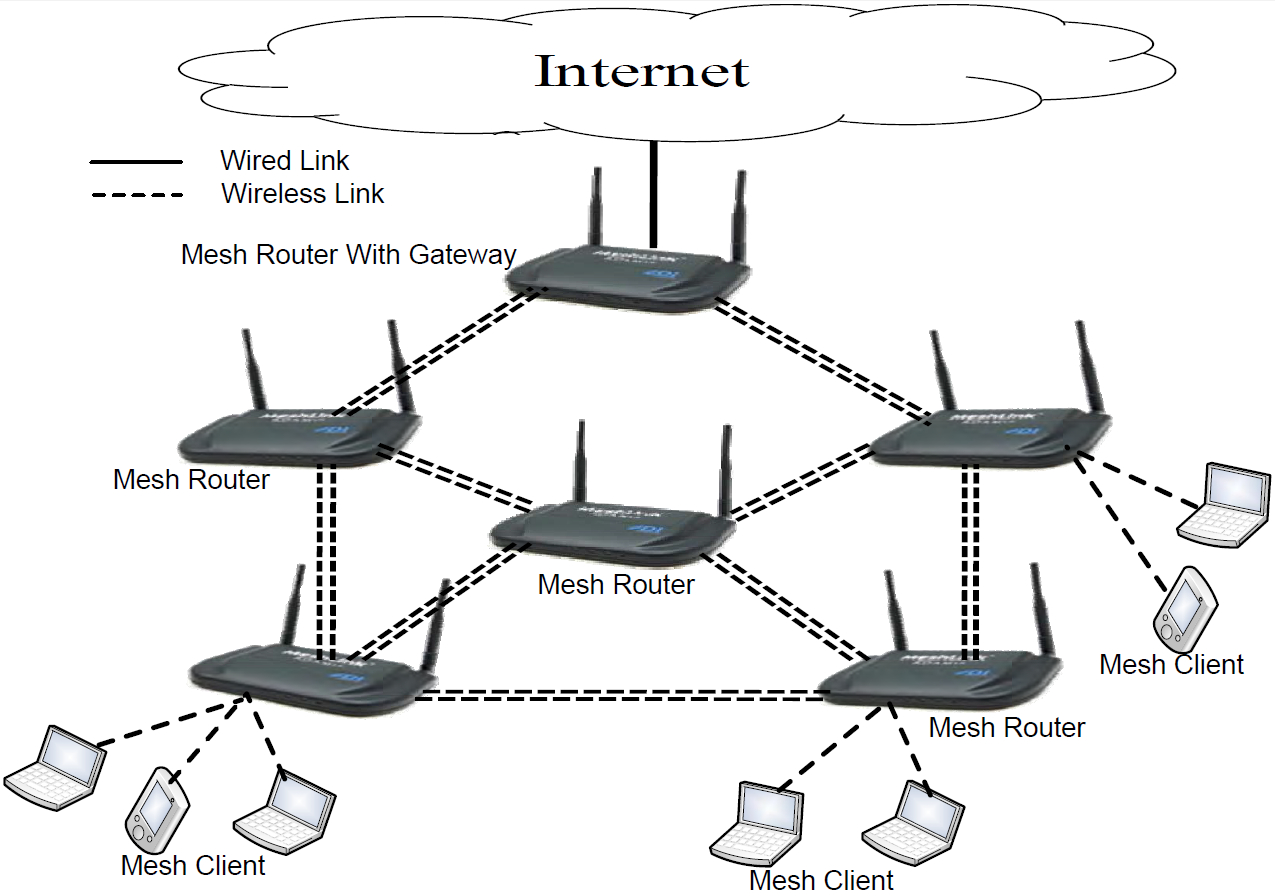
\includegraphics[width=0.8 \linewidth]{Images/wmn11.jpg}}
\captionof{figure}{Wireless Mesh Network Example}% only if needed
\caption*{http://www.intechopen.com/source/html/37888/media/wmn11.jpg}
\label{city}
\end{minipage}
\nocite{WMNs}
\clearpage

Then, we can say that WMN are a subtype of mesh networks. They have all the properties of these networks with the only difference that all the nodes are connected wirelessly. 

\subsection{Operating modes}
\nocite{qmpPresentation}

Mesh networks can operate in two different modes: Infrastructure mode and Ad-Hoc mode.

\begin{itemize}
	\item \textbf{Infrastructure Mode: }In this mode we have a central point named \ac{AP} that creates a \ac{BSS} zone in which all the packets have to go through the AP. This zone is identified by the MAC address of the AP, which is called BSSID in this context. Furthermore, we can say that a master/slave model is followed in infrastructure mode.
	
		\noindent%
\begin{minipage}{\linewidth}
\vspace{10 mm}
\makebox[\linewidth]{%
  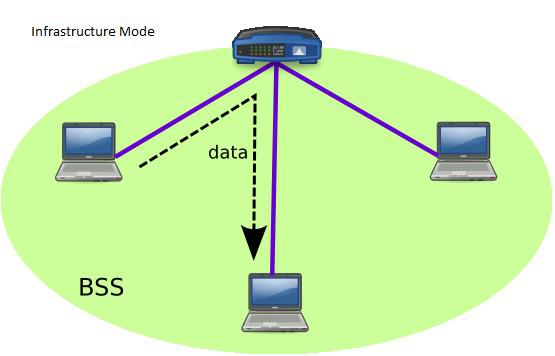
\includegraphics[width=0.8 \linewidth]{Images/InfMode.png}}
\captionof{figure}{Infrastructure Mode BSS}% only if needed
\caption*{\cite{qmpPresentation}}
\label{Infrastructure}
\end{minipage}

\clearpage
	\item \textbf{Ad-Hoc Mode: }In Ad-Hoc mode, all the participants play the same role. Therefore, every single node connects with all the nodes it can, and so the central point idea disappears. To identify which participants are in the same network we just need to find those who have the same BSSID. At this point, all the machines directly connected can exchange information but, a layer 3 routing protocol is required to allow the communication between nodes which are not connected directly. 
	
	\noindent%
\begin{minipage}{\linewidth}
\vspace{10 mm}
\makebox[\linewidth]{%
  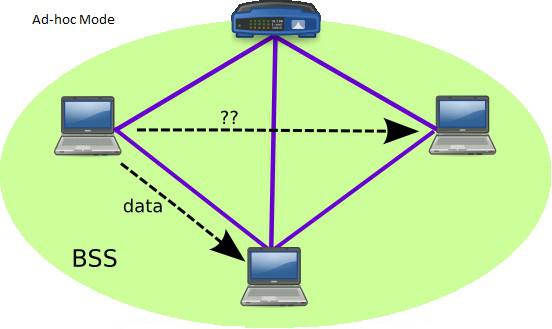
\includegraphics[width=0.8 \linewidth]{Images/AdhocMode.png}}
\captionof{figure}{Ad-Hoc Mode BSS}% only if needed
\caption*{\cite{qmpPresentation}}
\label{Ad-hoc}
\end{minipage}
\end{itemize}

\subsection{MANET Networks}

\ac{MANET} is a subtype of a mesh network. That is to say, when we have a mesh network which uses a wireless system to interconnect the nodes and is built in Ad-hoc mode, we talk about \ac{MANET}. Another way to define it can be: A \ac{MANET} network is a \ac{WMN} which operates in Ad-Hoc mode. 
\\[12pt]

Usually, when we talk about \ac{MANET} we are also referring to networks which have a self-configuring property. This property relies on the fact that the routers within the network are free-to-move anytime and to anywhere. A good definition could be this:
\\[12pt]

"\textit{A Mobile Ad hoc NETwork (MANET) is a kind of wireless ad-hoc network, and is a self-configuring network of mobile routers (and associated hosts) connected by wireless links - the union of which forms an arbitrary topology.}"\cite{Manetdef}
\\[12pt]


\section{Open \ac{MANET} Networks in Barcelona}

Nowadays, in Barcelona (and in some other cities) some MANET networks are being deployed. We will study this case in particular because is the one we are more familiar with. In general terms, all the deployments work in the same manner and so, studying one single case can give us a general a idea of all of them.
\\[12pt]

Normally, all these deployments only differ in some points, these are the more relevant ones:

\begin{itemize}
	\item The funding scheme
	\item The kind of hardware
	\item The firmware used 
\end{itemize}


\subsection{Funding scheme in Barcelona's \ac{MANET} networks}

There are some examples of MANET networks successfully deployed in Barcelona:

\begin{itemize}
	\item Gr�cia
	\item Sants
	\item Poble Nou
	\item Sant Joan Desp�
\end{itemize}


All these networks have been deployed using the same funding scheme, promoted by the Guifi.net foundation, and is, somehow, based on crowd-funding. Basically, anyone can install a new node and join to the mesh. There is just one restriction: you have to have direct vision with, at least, another node in the network. If you achieve this requirement, you can buy and install the node yourself and you expand the network. So, this is crowd-funding because every person joining the network funds its own equipment, which has the only requirement of being compatible with the firmware used. Since many people has no experience on installing and configuring the nodes, and despite the fact that both the hardware and software are specially designed to allow non-technical people to use it without problems, the foundation provides technical support for those who do not achieve in the installation. 

\subsection{The Kind of hardware in Barcelona's \ac{MANET} networks}

Being that the users are the owners of the network and so, the people who buy the equipment, usually low-cost hardware is used. Low-cost does not mean, low-quality, in fact some of the hardware used have very high features and a very good performance. Normally, the hardware used is from Ubiquity Networks (NanoStation, Rocket, Bullet, etc.), but it is not strictly necessary. Actually, any hardware compatible with the linux distribution openWRT is accepted. 
\\[10pt]

There are more information about some of this devices in Appendix 2.

\subsection{The Firmware used in Barcelona's \ac{MANET} networks}

This is maybe the most important difference between all the deployments around the world. In most of them, there is a common point: all the firmwares are openWRT based, but they have some differences. Particularly, in Barcelona the first deployments used the \ac{GSF} firmware, developed since 2003 for the Gracia Sense Fils Wireless Community\footnote{More information at: http://graciasensefils.net/}. Some year later, the firmware became outdated since the protocol versions where old and the configuration of the nodes was hard. Then, they decided to create a new firmware with bigger scope, they named it \ac{QMP} and is the one being used currently (some nodes have to be migrated to \ac{QMP} yet).
\\[12pt]

\ac{QMP} has been chosen in Barcelona because is a firmware that covers perfectly the needs in the deployments carried out there, and has been developed by themselves. Nowadays, in most of the deployments a new firmware is designed specially for them, and despite the fact that many of them could be used in other deployments, it does not normally happen. It is not an efficient way to work, and because of it a new initiative has just started, it is called "libre-mesh"\footnote{More information at: http://libre-mesh.org/}. This initiative tries to build a new firmware based on three existent ones: QMP (Spain), AlterMesh (Argentina) and eigenNet (Italy). It can be a good opportunity to merge all the best points of every firmware a create a new version that fits in many different scenarios.

\section{\ac{QMP} firmware basics}

\subsection{Main Features}

\ac{QMP} \footnote{ http://qmp.cat} is an Operating System designed for embedded devices, a firmware. The main features of this firmware are:


\begin{itemize}
	\item OpenWRT based
	\item 802.11a/b/g/n support
	\item IPv6 native
	\item IPv4 tunneled over IPv6
	\item Auto configuration system
	\item Web GUI to monitor and configure
	\item Visualization tools (maps, graphs, etc.)
	\item Automatic dynamic routing  (zero-conf)
	\item BGP (Border Gateway Protocol) support
	\item Open Source 
\end{itemize}

\subsection{Quick Deployments}

\ac{QMP} has been specially designed and developed to achieve quick network deployments. To do so, they have created the auto configuration feature which plays a very important role within the firmware. When we talk about quick deployments, we mean that we have to accomplish these requirements:
 
 \begin{itemize}
	 \item The deployment must be performed as fast as possible.
	 \item It must be able to be done by non-technical people.
	 \item It must be possible in most situations.
\end{itemize}

\subsection{Addressing}

\ac{QMP} uses three different kind of IP addresses:

\begin{itemize}
	\item IPv6 ULA: IPv6 private range to be used internally in the mesh. These IPs are used for the communication among the nodes in the mesh network, and so they are not neither valid nor routable outside.
	\item IPv6 RIPE: IPv6 public IPs range (6to6 tunneling). These are globally valid and routable.
	\item IPv4: IPv4 private range to connect with the final user (4to6 tunneling). They are assigned to the final users attached to a node in the mesh, when 	they transmit any packet that has to travel throughout the mesh it is encapsulated in an IPv6 packet (tunneling).
\end{itemize}


\noindent%
\begin{minipage}{\linewidth}
\vspace{10 mm}
\makebox[\linewidth]{%
  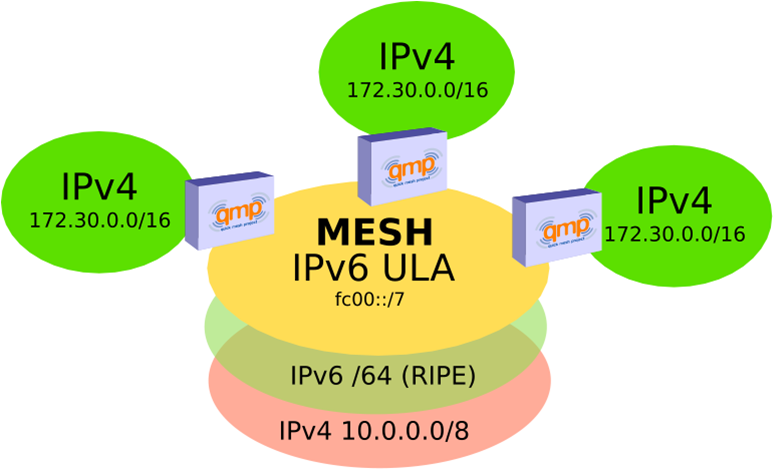
\includegraphics[width=0.8 \linewidth]{Images/qmpAddr.png}}
\captionof{figure}{QMP Addressing}% only if needed
\caption*{\cite{qmpPresentation}}
\label{AddrQMP}
\end{minipage}

\subsection{Operating modes}

The firmware has two different operating modes, depending on the scenario we should choose one or the other:


\begin{itemize}
	\item Roaming for fast deployments: All the access points in this mode will have the same IP and the same ESSID in order to allow users mobility, namely, they will not lose the connection although they switch from an \ac{AP} to another. Every AP implements a \ac{NAT} and so, two users attached to different \ac{AP}s will not have direct vision between them.

	\item Community: Every node will have a randomly assigned IPs range and will announce this range through the mesh. There is not \ac{NAT}, every user has direct vision with the others (1 hope away from the IPv4 network layer point of view), but mobility is not allowed (no roaming).
\end{itemize}


\noindent%
\begin{minipage}{\linewidth}
\vspace{10 mm}
\makebox[\linewidth]{%
  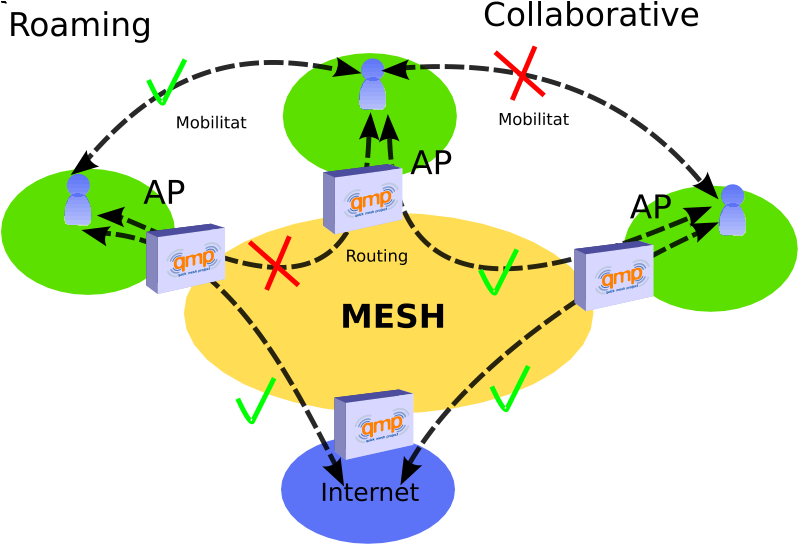
\includegraphics[width=0.8 \linewidth]{Images/qmpModes.png}}
\captionof{figure}{QMP Operating Modes}% only if needed
\caption*{\cite{qmpPresentation}}
\label{ModesQMP}
\end{minipage}


\subsection{\ac{DRP}}

The firmware uses different protocols:


\begin{itemize}
	\item  \ac{BMX6} as the main \ac{DRP}.
  \item  \ac{OLSR6} as a backup \ac{DRP}.
  \item  Babel as a backup \ac{DRP} but optional. 
\end{itemize}

Usually, two networks are built in parallel the main one using \ac{BMX6} and the backup on using \ac{OLSR6}. There are two reasons for that:

\begin{enumerate}
	\item To prevent that a node gets isolated (no neighbors) due to a single \ac{BMX6} failure. 
	\item To make performance measurements of both protocols in exactly the same environment. This was very useful at the beginning of the project to decide which protocol was better in every scenario.
\end{enumerate}


All these three protocols use IPv6 ULA to talk to other nodes and are isolated at the link layer (MAC) using VLANs. It allows the protocols to work in parallel (if necessary) without interfering with the other protocols. 


\subsection{\ac{BMX6}}

Since \ac{BMX6} is the main \ac{DRP} we are going to analyze it deeply:
\\[10pt]

\textit{\ac{BMX6} is a table-driven routing protocol for wireless mesh networks. [...] its goal is to compose a path from source to destination by deciding on each node which will be the next hop. \ac{BMX6} is a distance vector protocol, since the information each node manages is [...] destination node, next hop and cost. } \cite{Bmx6}
\\[12pt]

In terms of dissemination - how the nodes exchange the information - we can distinguish between two different states: transient and steady. 


\begin{itemize}
	\item Transient phase: the nodes exchange information related to the environment: \ac{IID}, nodes description, links, etc. Thanks to this information, ever single node builds a dictionary table that translates between \ac{IID} to the global hashes of the full node description.
	\item Steady phase: every node has local information state (\ac{IID}-to-hash dictionary) and global information state as hash-to-description.  So, during this phase there is just a small exchange of packets that inform about link metrics and network changes. Thank to the tables set up in transient phase, those packet do not need to use the 128 bit IPv6 address as the identifier, they can use the 16 bit \ac{IID} which produces a much lower overhead. 
\end{itemize}

To summarize, we can say say that \ac{BMX6} controls the overhead better than other protocols (some experiments demonstrate that, for example: \cite{Bmx6}) there is a big overhead at the very beginning (transient state) and later it becomes very low during the steady state. So the main features of this protocol are:


\begin{itemize}
	\item Pro-active: Uses UDP flooding to periodically send Originator Messages (OGM) and build a routing table.
	\item Destination-sequenced, Distance-vector (DSDV): 		Every node just knows which neighbor is better to reach another, namely, they do not need to know the entire topology, just the best paths.
	\item Does not use IP as node identifier, it uses global identifiers using SHA2 hashing. 
\end{itemize}


In terms of the kind of frames used by \ac{BMX6} we have two different types:  periodic messages, periodically generated on every node and occasional messages, exchanged only when necessary. The most used are the periodical which are the following:
\\[12pt]

\noindent%
\begin{minipage}{\linewidth}
%\begin{center}
\begin{tabular}{| c | p{0.8\linewidth} |}
\hline \textbf{Frame name} & \textbf{Description} \\
\hline HELLO\_ADV & Hello advertisement. Used for letting neighboring nodes detect the link quality in transmit direction (from sending to receiving node).\\
\hline RP\_ADV & Rx probe advertisement. Used for reporting about reception rate of hello messages from neighboring nodes.\\
\hline OGM\_ADV & OGM advertisement. Used for updating periodically route and metric information over the mesh.\\
\hline OGM\_ACK & OGM acknowledgment. Used for acknowledging the previously reception of a full OGM\_ADV frame.\\
\hline
\end{tabular}
\captionof{table}{BMX6 Frames}
\caption*{\cite{paupfc}}
\label{table:bmx6_frames}
%\end{center} 
\end{minipage}
  
\chapter{Contribution}

As we mentioned in previous chapters, we wanted to find ways to contribute to current open mesh networks, by providing ideas, introducing new hardware (or new ways to use the existing one) or building applications that run over the network.
\\[12pt]

We can divide the contribution of this project in three different points:


\begin{enumerate}
	\item Study and documentation of the Mobile Node project
	\item Installation of a node within Poblenou Mesh
	\item Development of an audio and/or video streaming Android application
\end{enumerate}


\section{Mobile Node Project}

\nocite{efrainMedia}
The mobile node is a portable and auto-configurable transmission unit with wireless technology that offers mobility in the urban space. This node is designed to contribute to the digital mesh through existing networks. Furthermore, it provides connectivity with a wide range of different hardware: fixed nodes, other mobile nodes, smartphones, pc, tablets, etc.
\\[12pt]

The basic idea that lies behind the concept of the mobile node, is the socialization and modeling of the networks according to the interests and needs of communities and citizens, completely changing the paradigm. At present, networks are designed and deployed based on corporate and/or government interests, this fact does not allow the home user to control its data flows and, much less, get involved in the process.
\\[12pt]

In other words, what we are doing with the Mobile Node, is making the most of the hardware and firmware we have, combining them and using the resulting device in a different way. So, a mobile node, in our context, is a device that can be used to expand networks already deployed and give coverage to a zone where there was no coverage at this time. Therefore, we are taking advantage of the "Auto-configuration" feature of \ac{QMP} to provide Internet Access rapidly.
\\[12pt]

The main advantage of this device, is the speed and freedom that offers. Given this features, the most common usage	will be as a temporary solution to cover a particular zone during a certain period of time. It can be very useful in events, congresses, concerts, parties, etc. Which will  take just a few hours or days. Using this device in cities like Barcelona, where fixed mesh networks are quite extended, will allow the organizers of the events to provide Internet Access to the attendants in a very fast, easy and cheap manner. 
\\[12pt]

Although covering events is, perhaps, the main usage we can give to our mobile node it is not the only one. Since we are talking about open networks, with open firmware we have the freedom to use them as we prefer. Normally, the mobile nodes are supplied using batteries which will last just some hours, but it is not strictly necessary to use them that way. We could join a community or create a new one and model our own networks using mobile nodes, there are no restrictions considering that a mobile node is nothing but the same hardware and the same firmware used in a different way. 
\\[12pt]

Given all these facts, that is the reason why we talk about changing the paradigm and start modeling the networks according to the interests of those who are going to use them.
\\[12pt]

So, the biggest contribution we did in that field, was to write a document talking about the project, its origins, how to build our first mobile node, the hardware we need, how to configure some devices and build a small mesh, the prototypes that are being tested nowadays, etc. Since this is a project which is being carried out by Efra�n Foglia with the support of Mobility Lab, we just took all the information and started doing experiments to build the networks and the nodes, but did not do anything new. So we created a document gathering all the information that will allow beginners to start learning and working in that field. This document can be found at appendix 2.    

\chapter{Results}
TODO
\chapter{Conclusions}
TODO
\chapter{Future Work}
TODO






\bibliography{bibliography}
\cleardoublepage

\chapter{Appendixes}
\appendix

\section{Appendix 1: Pilot Charter}
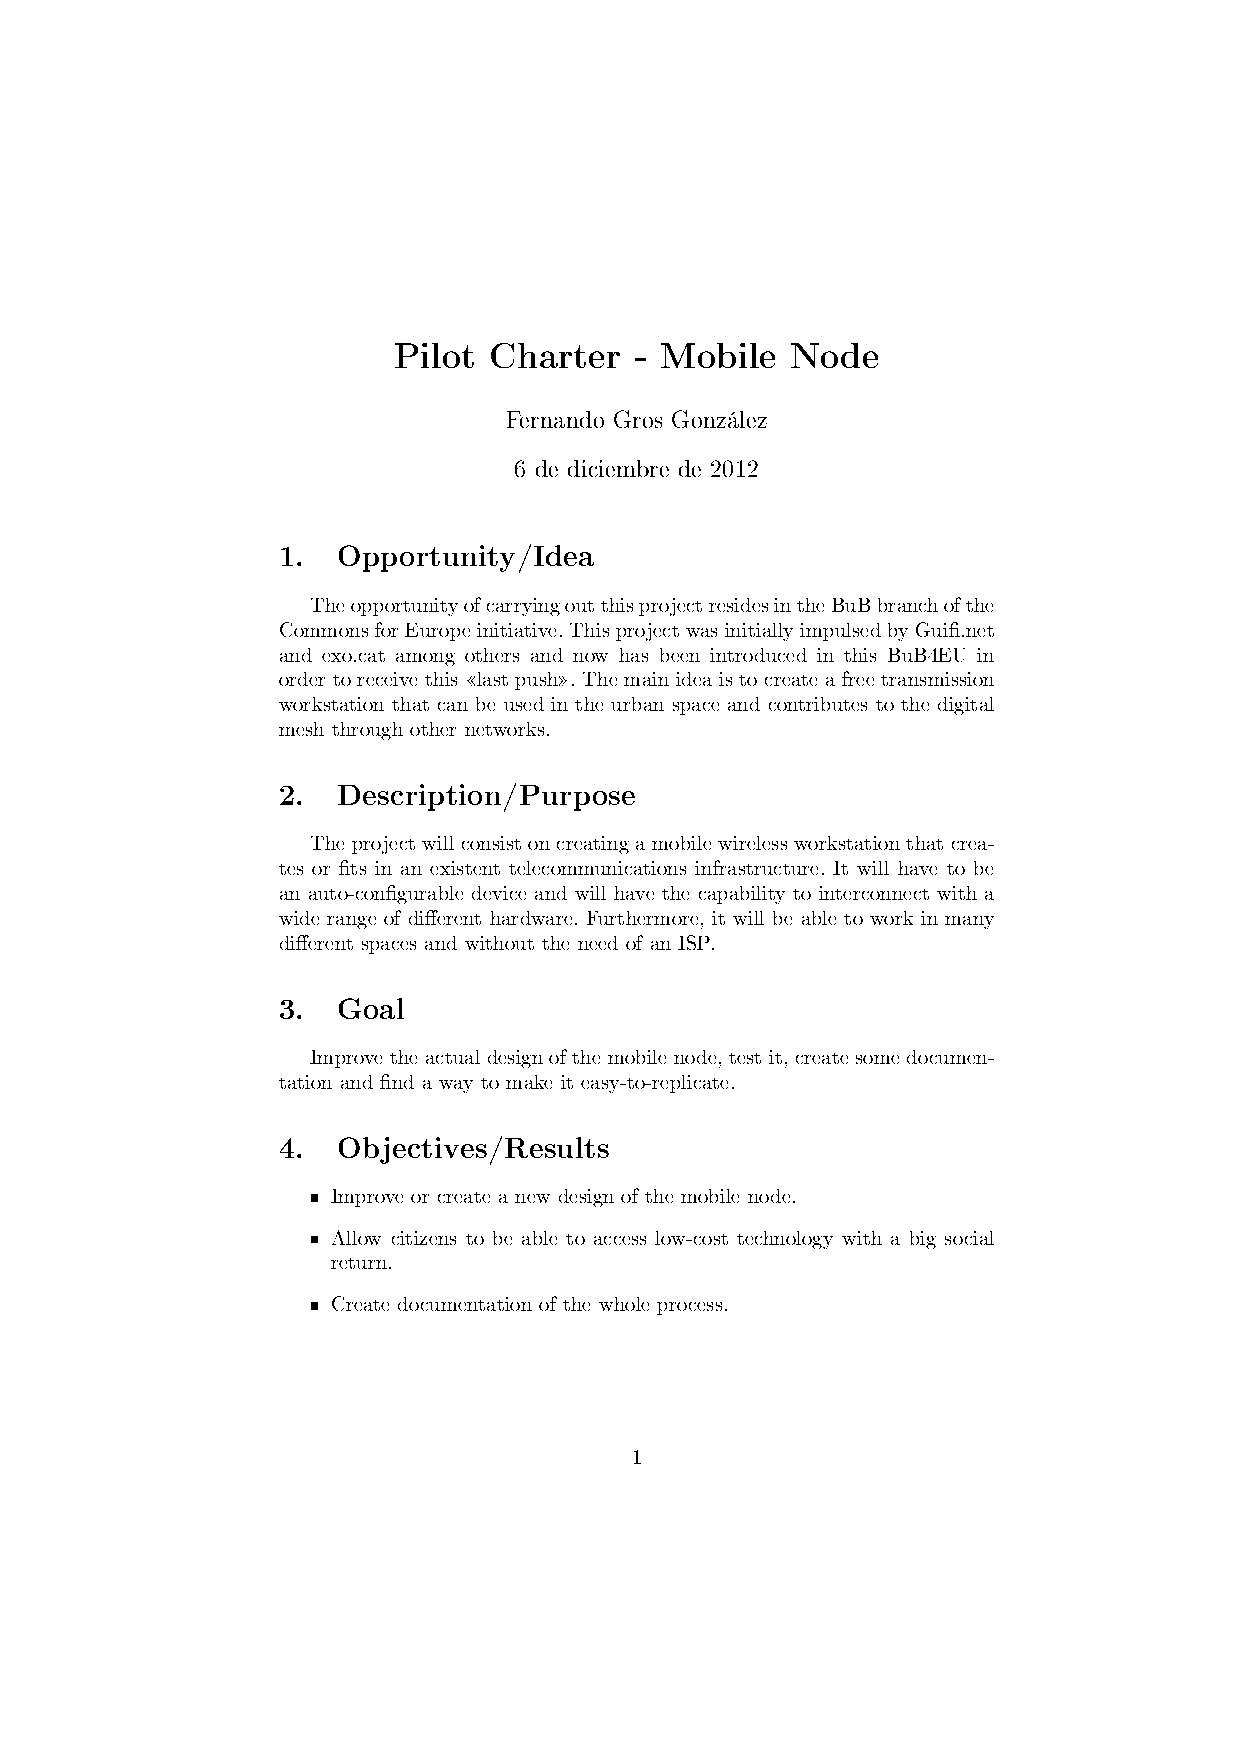
\includepdf[pages={-}]{Appendix/projectcharterMN.pdf}

\section{Appendix 2: Documentation}
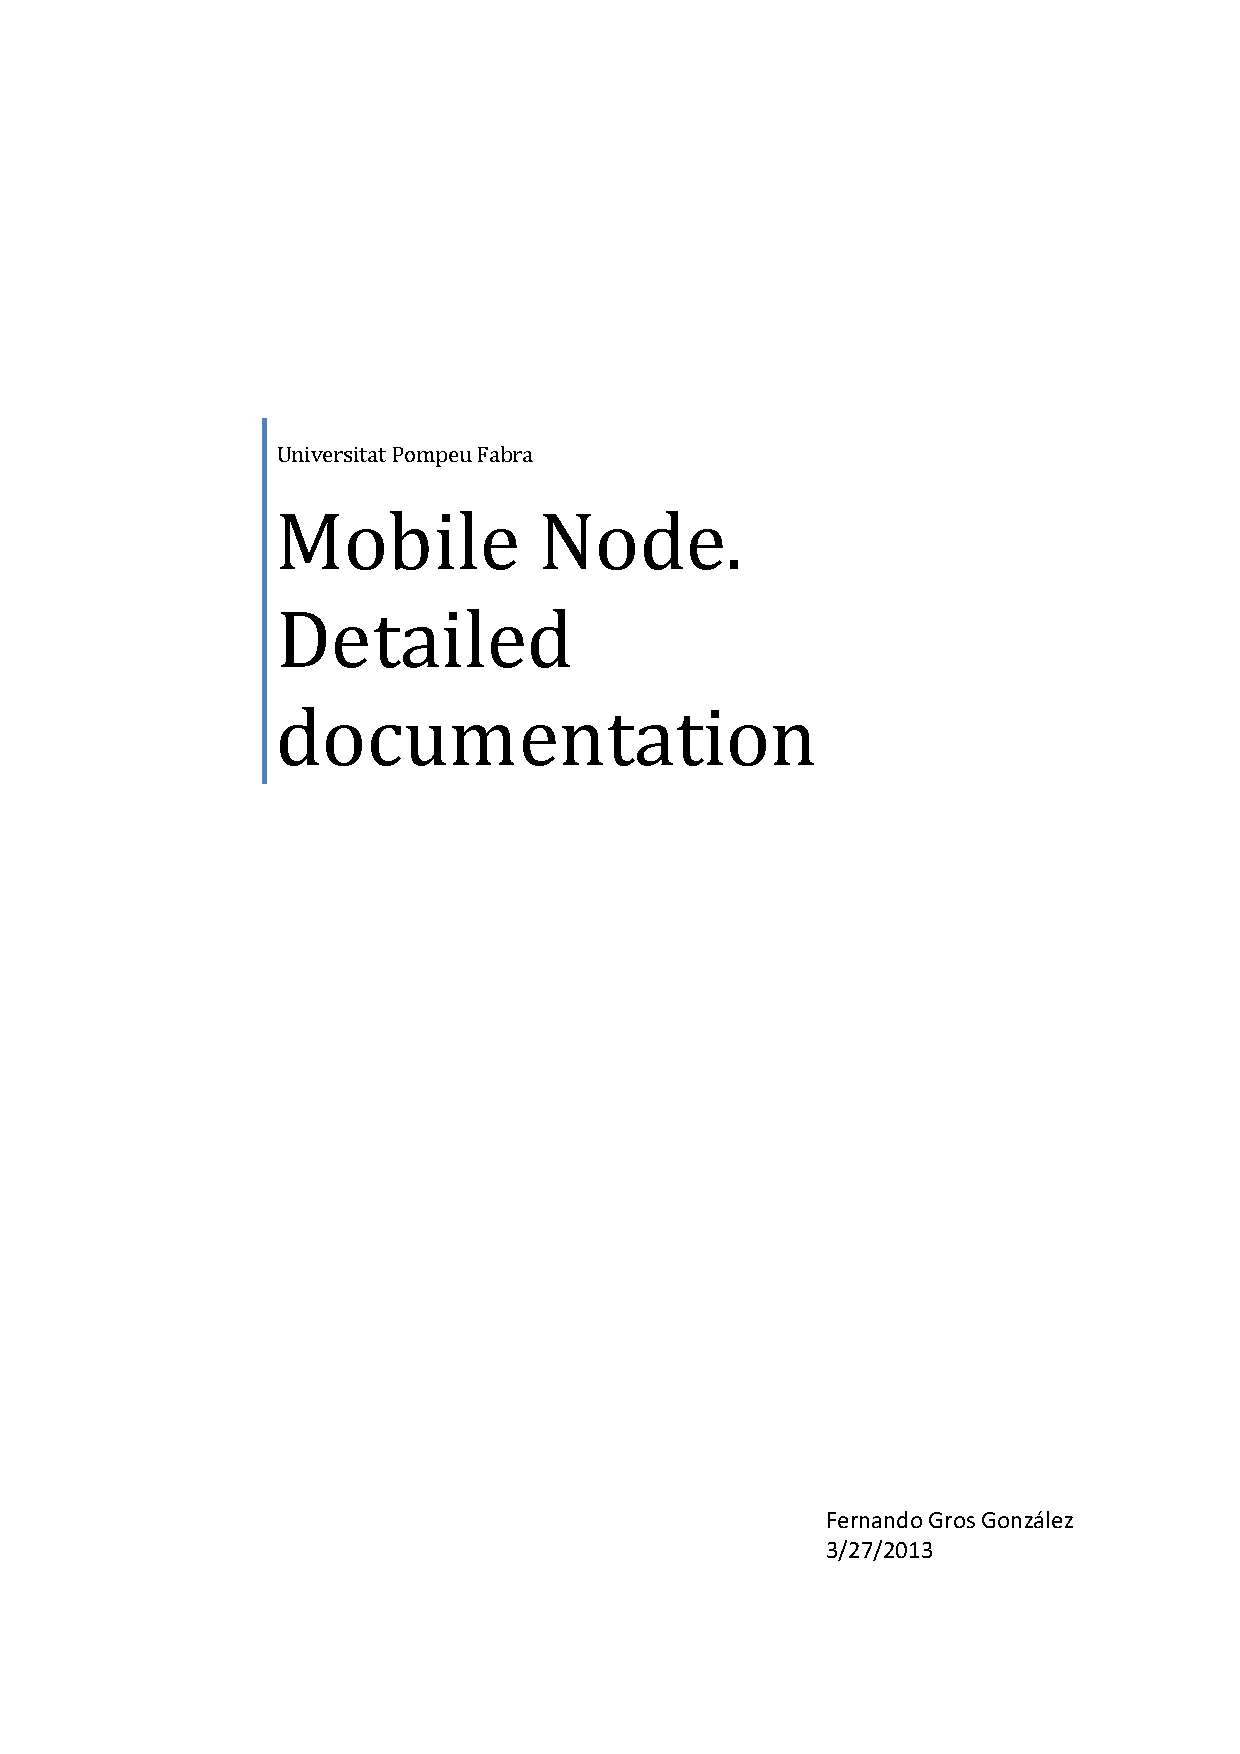
\includepdf[pages={-}]{Appendix/Documentation.pdf}

\section{Appendix 3: QMP Presentation}
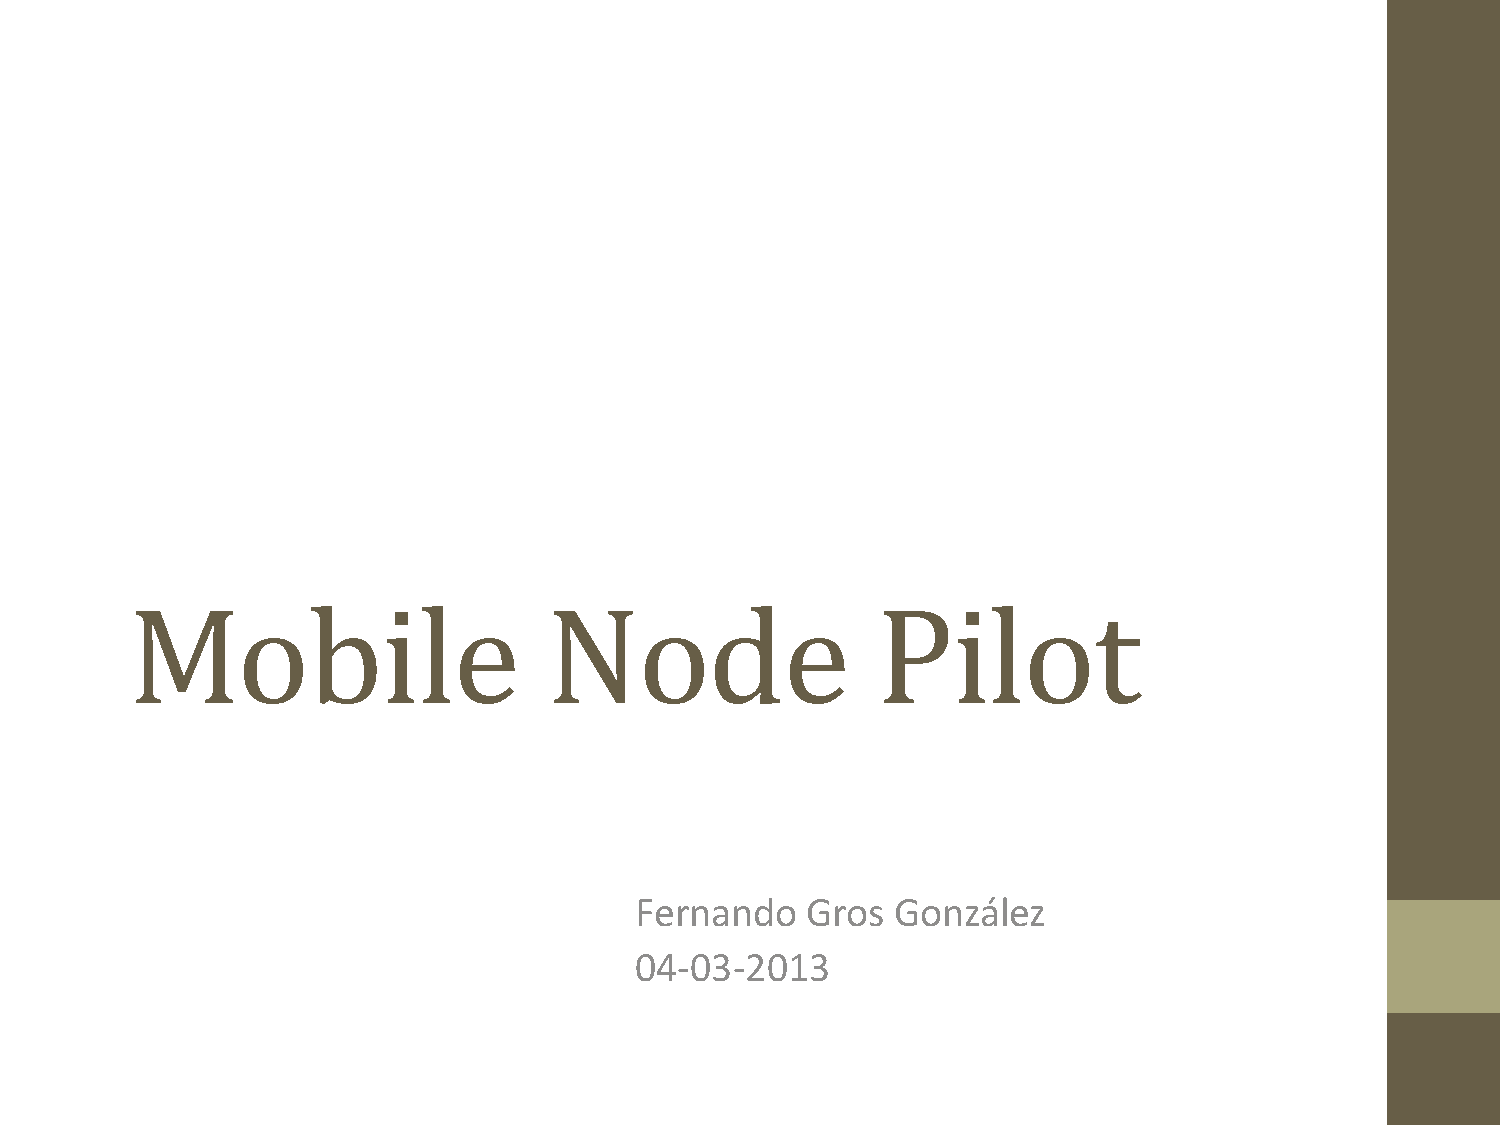
\includepdf[pages={1-19}]{Appendix/QMPDemo.pdf}



\backmatter
\printindex





\end{document}


%NUMERACI� DE LA P�GINA EXTERIOR EXCEPTE EN LA PRIMERA P�GINA DE CADA CAP�TOL
\usepackage{fancyhdr}
\pagestyle{fancy}
\fancyfoot{}
\fancyfoot[RO]{\thepage}
\fancyfoot[LE]{\thepage}


%MUTIPLES �NDEX
%En el pre�mbul
\usepackage{multind}
\makeindex{authors}
%Introducci� d'entrades la forma
\index{authors}{Einstein}
%Situaci� de l'�ndex
\printindex{authors}{Author index}
%Cal eliminar les comandes \usepakage{makeidx} \makeindex \printindex
%cal exacutar des de la l�nia de comandes makeindex authors